\documentclass{article}
\usepackage[top=0.75in, bottom=0.75in, left=1.25in, right=1in]{geometry} % formatage
\usepackage[frenchb]{babel}
\usepackage[utf8]{inputenc} 
\usepackage{amsmath} % pour utiliser des maths de base 
\usepackage{amssymb} % pour faire \mathcal{}=>des lettres ''cursives''
\usepackage{amsthm} % La petite boîte de fin de preuve
\usepackage{graphicx} % pour importer des images...http://www.tex.ac.uk/cgi-bin/texfaq2html?label=figurehere
\usepackage{titlesec} % automatique, pour faire des sous-titres moins laids
%\usepackage{cancel}
\usepackage[procnames]{listings}
\usepackage[T1]{fontenc}        % http://tex.stackexchange.com/questions/11897/draw-a-diagonal-arrow-across-an-expression-in-a-formula-to-show-that-it-vanishes%
\usepackage[squaren]{SIunits}
\usepackage{subcaption} % Avoir plusieurs sous-figures (graphiques) dans une figures et pouvoire les étiqueter
\usepackage{color}
\usepackage{lipsum}
\usepackage{caption}
\usepackage{enumitem} % Permet d'avoir plus de flexibilité dans les enumerations.
\usepackage{wasysym} 
\usepackage{braket}
\usepackage{mathtools}
\usepackage{multirow} % Fusionner des lignes dans un tableau
\usepackage{mathrsfs} % Faire le symbole de la transformée de Laplace
\usepackage{bbm}
\usepackage{array}
\usepackage{diagbox} % diagonale dans les tableaux
\usepackage{dsfont} % Faire des belles indicatrices                         
\usepackage{float} % placer les tableaux et images où tu veux
\usepackage{listings}
\usepackage[utf8]{inputenc}
\usepackage{comment}
\usepackage{pst-node}
\usepackage{fancyvrb} % Les varbatims gardent l'indentation
\usepackage{enumitem}
\usepackage{breakcites} % Faire en sorte que les citations ne sortent pas dans la marge
\usepackage{graphicx} % Insérer des graphiques
\usepackage{pgfplots}
\usepackage{hyperref} % Faire des hyperliens
\usepackage{verbatim} % Inclure un fichier .text en verbatim
\usepackage{xcolor}
\pgfplotsset{width=10cm, compat=1.9}

% Changer la couleur des hyperliens
\hypersetup{colorlinks = true,
	allcolors  = blue, % default color = black
	%	citecolor  = black
}  


% redefine \VerbatimInput
\RecustomVerbatimCommand{\VerbatimInput}{VerbatimInput}%
{fontsize=\footnotesize,
	%
	frame=lines,  % top and bottom rule only
	framesep=2em, % separation between frame and text
	rulecolor=\color{Gray},
	%
	label=\fbox{\color{Black}data.txt},
	labelposition=topline,
	%
	commandchars=\|\(\), % escape character and argument delimiters for
	% commands within the verbatim
	commentchar=*        % comment character
}


\newcommand{\RomanNumeralCaps}[1]
    {\MakeUppercase{\romannumeral #1}}

\newtheorem{lemme}{Lemme}
\newtheorem{preuve}{Preuve}
\newtheorem{code}{Code informatique}
\newtheorem{exemple}{Exemple}
\newtheorem{scenario}{Scénario}
\newtheorem{algo}{Algorithme}
\newtheorem{definition}{Définition}
\newtheorem{proposition}{Proposition}
\newtheorem{propriete}{Propriété}
\newtheorem{test_hypothese}{Teste d'hypothèse}

\begin{document}
	\renewcommand{\tablename}{Tableau}
	\renewcommand{\figurename}{Illustration}
	\renewcommand{\P}{\mathbb{P}}
	
	\begin{titlepage}
		\centering % Centre everything on the title page
		
		\scshape % Use small caps for all text on the title page
		
		\vspace*{7\baselineskip} % White space at the top of the page
		
		%------------------------------------------------
		%	Title
		%------------------------------------------------
		
		\rule{\textwidth}{1.6pt}\vspace*{-\baselineskip}\vspace*{2pt} % Thick horizontal rule
		\rule{\textwidth}{0.4pt} % Thin horizontal rule
		
		\vspace{0.75\baselineskip} % Whitespace above the title
		{\LARGE Travail pratique 1\\} % Title
%		\vspace{0.75\baselineskip}
		\vspace{0.75\baselineskip} % Whitespace below the title
		
		\rule{\textwidth}{0.4pt}\vspace*{-\baselineskip}\vspace{3.2pt} % Thin horizontal rule
		\rule{\textwidth}{1.6pt} % Thick horizontal rule
		
		\vspace{4\baselineskip} % Whitespace after the title block
		
		%------------------------------------------------
		%	Subtitle
		%------------------------------------------------
		
		Travail présenté à \\
		{\scshape\Large M. Thierry Duchesne\\}
		
		\vspace*{4\baselineskip}
		
		Dans le cadre du cours\\
		{\scshape\Large Théorie et applications des méthodes de régression \\ STT-7125}
		
		% Subtitle or further description
		
		\vspace*{4\baselineskip} % Whitespace under the subtitle
		
		%------------------------------------------------
		%	Editor(s)
		%------------------------------------------------
		
		Réalisé par l'équipe 7:\\
		{\scshape\Large Alexandre Lepage\\
		\& Amedeo Zito} % Editor list
		
		\vspace*{5\baselineskip}
		
		le 2 novembre 2020
		
		\vspace{0.4\baselineskip} % Whitespace below the editor list
		
		\vfill % Whitespace between editor names and publisher logo
		
		%------------------------------------------------
		%	Publisher
		%------------------------------------------------
		
		
\includegraphics[height=1.2cm]{UL_P.pdf}\\
		
		Faculté des sciences et de génie\\
		École d'actuariat\\
		Université Laval
		
		\vspace*{3\baselineskip}
		
	\end{titlepage}
	
%	\pagenumbering{Roman} % Pagination en chiffres romains
%	\setcounter{page}{0} 
%	
%	\newpage
%	\strut % Page blanche
%	\newpage
%	
%	\tableofcontents
%	\renewcommand{\listfigurename}{Liste des illustrations}
%	\newpage
%	
%	\listoffigures
%	\listoftables
%	\newpage
%	
%	\pagenumbering{arabic} % Pagination en chiffres normaux
%	\setcounter{page}{1}


\section{Introduction}
Les méthodes de régression linéaires sont fort utiles afin d'identifier des variables pouvant expliquer un comportement ou un phénomène et elles peuvent s'avérer efficaces pour faire de la prédiction si les données disponibles sont appropriées.\\

L'objet de ce travail est d'expérimenter l'utilisation de cette famille de modèles afin de résoudre trois problèmes de nature différente. 
%
La premier d'entre eux consiste à réaliser une régression linéaire afin de prédire le taux de mortalité à partir de variables mesurant la pollution environnementale et les caractéristiques socio-démographiques de 60 localités.
%
Le second problème consiste à utiliser un modèle de régression afin de définir les facteurs associés à une hausse du risque d’un diagnostic positif de maladie coronarienne.
%
En ce qui a trait au dernier problème, celui-ci s'inscrit dans un contexte d'assurance automobile et consiste à construire un modèle visant à voir s’il y a une association entre les caractéristiques du véhicule et de l'assuré et le nombre de réclamations.


\section{Analyse et traitement de la multicollinéarité}\label{sect_multicollinearite}
La force des modèles de régression linéaire provient de l'hypothèse que la matrice de schéma $\boldsymbol{X}$ est de plein rang; c.-à-d. qu'aucune colonne n'est linéairement dépendante des autres colonnes. Ce faisant, on s'assure qu'il n'existe qu'un seul inverse possible à la matrice $\boldsymbol{X}'\boldsymbol{X}$; de ce fait, on s'assure également que le vecteur des paramètres du modèle $\hat{\boldsymbol{\beta}}$ soit unique (un seul minimum à la fonction de perte utilisée pour l'entraînement). Ainsi, s'il existe un problème de multicolinéarité, il en découlerait que la matrice de schéma $\boldsymbol{X}$ ne serait plus de plein rang et il pourrait exister plusieurs minimum locaux à la fonction de perte utilisée pour entraîner le modèle. Il en résulterait alors une instabilité dans la convergence des paramètres et la variance de certaines de ces composantes serait démesurément grande.
%
Pour cette raison, avant même de réaliser la sélection de modèle pour chacune des étapes, il faut d'abord mesurer le degré de multicollinéarité entre les potentielles variables explicatives disponibles.\\

Un outil bien pratique pour détecter la présence de multicollinéarité est le facteur d’inflation de la variance (VIF). Ce dernier peut être calculé avec la fonction \texttt{ols\_vif\_tol()} du \textit{package} \texttt{olsrr} en \texttt{R}. Cependant, si les données utilisées comportent une ou plusieurs variables catégorielles, cette mesure n'est plus adéquate (voir \cite{fox1992generalized}). Dans ce cas, on préférera le facteur d'inflation généralisé (GVIF) et sa version standardisée: $(\mathrm{GVIF}_j)^{1/(2 p_j)}$ , où $p_j$ correspond au nombre de degrés de libertés (le nombre de paramètres) rattachés à la $j^\mathrm{e}$ variable explicative du modèle, $j\in \{1,\dots,p'\}$. 
À noter que lorsque $p_j=1$, alors $\mathrm{GVIF}_j = \mathrm{VIF}_j$.
%
Afin de mesurer cette métrique, Fox et Monette ont créé la fonction \texttt{vif} du \textit{package} \texttt{car}. De façon générale, plusieurs auteurs suggèrent de considérer que $\mathrm{VIF_j}>10$ pourrait signaler un problème de multicolinéarité. En suivant cette logique, on peut considérer qu'il y a problème de multicolinéarité si $(\mathrm{GVIF}_j)^{1/(2 p_j)} > \sqrt{10} \approx 3.16,$ pour $j=1,\dots,p'$.\\

Si, effectivement, un problème de multicolinéarité est détecté, alors la fonction \texttt{ols\_eigen\_cindex()} du \textit{package} \texttt{olsrr} permet de faire un diagnostique plus approfondi. En effet, cette fonction permet de calculer les valeurs propres (\textit{eigen values}) associées à la matrice des coefficients de corrélation échantillonnaux $\boldsymbol{X^{\star}}'\boldsymbol{X^{\star}}$. 
%
À partir de celles-ci, elle calcule des indices de conditionnement définis comme
$$\phi_j = \sqrt{\frac{\lambda_{max}}{\lambda_j}},\ j=1,\dots,p',$$
où $\lambda_j$ correspond à la $j$-ème valeur propre de $\boldsymbol{X^{\star}}'\boldsymbol{X^{\star}}$ et $\lambda_{max}=\max(\lambda_1,\dots,\lambda_{p'}).$
Ces indices de conditionnement sont des indicateurs de la force de dépendance linéaire unissant certaines variables.
%
Ainsi, on regardera la ligne du tableau correspondant à la valeur de $\phi_j$ qui est la plus élevée. Une règle du pousse veut que si $\phi_j > 30$, alors on est en présence de multicolinéarité. Dans ce cas, on considérera la  proportion de la variance de $\hat{\beta}_l$ qui est expliquée par la $j$-ème dépendance linéaire, pour $l=1,\dots,p'$. C.-à-d. 
$$ p_{lj} = \frac{v_{lj}^2/\lambda_j}{c_{jj}},$$
où $v_{lj}$ correspond au $l$-ème élément du vecteur propre $\boldsymbol{v}_j$ associé à la $j$-ème valeur propre $\lambda_j$ et $c_{jj} = \sum_{l=1}^{p'}v_{lj}^2/\lambda_j$. 
Si $p_{lj} > 0.6$, alors on conclu que la $l$-ème variable explicative contribue à la $j^\mathrm{e}$ multicolinéarité et cause problème.\\

Dans ce cas, les solutions possibles consistent à appliquer une transformation non linéaire sur les variables explicatives (p.ex. transformation logarithmique ou racine carrée), réduire la dimension de la matrice de schéma en retirant la variable la plus problématique. S'il y a plusieurs valeurs de $l$ pour lesquelles $p_{lj}>0.5$ pour un même $j$, alors il est possible de les regrouper à l'aide d'une moyenne. Par exemple, pour $j=\underset{j\in\{1,\dots,p'\}}{\mathrm{argmax}}\{\phi_j\}$, si on a $p_{1j}>0.5$ et $p_{2j}>0.5$, alors on peut combiner $x_1$ et $x_2$ de la façon suivante: $(x_1+x_2)/2$.\\

Après avoir réalisé ces étapes, il faut recommencer itérativement ce processus jusqu'à ce qu'il n'y ait plus de problème soulevé par l'analyse du VIF ou du GVIF.


\section{Question 1}\label{sect_qst1}

	Pour la première question de ce travail, on considère un jeu de données présentant des variables mesurant la pollution environnementale et les caractéristiques socio-démographiques de 60 localités. L'objectif de cette question est de valider qu'il est possible de prédire la mortalité d'une région en fonction de ces variables explicatives et de donner un estimé ponctuel ainsi qu’un intervalle de confiance à 95\% sur une observation de donnée.
	
	\subsection{Traitement de la multicollinéarité}
	
	Pour atteindre cet objectif, la première étape consiste à réaliser une analyse de multicollinéarité telle que décrite dans la section \ref{sect_multicollinearite}. Se faisant, on découvre que les VIFs pour les variables A12 et A13 sont supérieures à 10. Afin de traiter ce problème, on peut commencer par regarder s'il est pertinent d'effectuer une transformation non linéaire de certaines variables explicatives. Afin de visualiser les options envisageable, les illustrations \ref{Qst1_transformations_1} à \ref{Qst1_transformations_5} présentent l'effet d'une transformation logarithmique (au centre) et celui d'une transformation racine carrée (à droite) sur la relation existant entre la variable endogène et chacune des variables explicatives. Si on voit que cette transformation améliore la relation de linéarité existant entre les variables en question, alors on procède à la transformation appropriée. Suite à l'analyse des illustrations \ref{Qst1_transformations_1} à \ref{Qst1_transformations_5}, on en vient à considérer que les variables A12 et A13 méritent à recevoir une transformation logarithmique, de même que les variables A9 et A14 profiteraient à recevoir une transformation racine carrée. Afin de valider ces observations, on teste différents modèles utilisant plusieurs combinaisons de transformations. Il advient que le modèle complet possédant l'AIC le plus petit est le suivant:
	\begin{align}\label{modele_complet}
		\mathrm{B} &\sim \mathrm{A1 + A2 + A3 + A4 + A5 + A6 + A7 + A8 + I(sqrt(A9))}\\
			&\mathrm{+ A10 + A11 + I(log(A12)) + I(log(A13)) + I(log(A14)) + A15}.\nonumber
	\end{align}
	
	Une fois que ces transformations sont effectuées, on refait l'analyse des VIFs. Puisque celle-ci nous indique que la multicollinéarité n'est toujours pas réglée, on procède aux étapes décrites dans la section \ref{sect_multicollinearite} après quoi on trouve le modèle suivant:
	\begin{equation}\label{modele_traitement_multicol_methode_iterative}
		\mathrm{B} \sim \mathrm{A1 + A2 + A8 + A11 + I(log(A14)) + I(log(sqrt(A12 * A13)))}.
	\end{equation}
	
	À titre comparatif, nous avons voulu tester s'il était possible d'avoir un modèle plus performant si le traitement de la multicolinéarité était fait par sélection de variables en utilisant une régression LASSO. Avec la fonction \texttt{glm.net} du \textit{package} du même nom et avec le paramètre \texttt{alpha=1}, on essaie plusieurs valeurs pour le terme de pénalité $\lambda$ en commençant par celui qui est le plus inclusif (lambda le plus petit). Ainsi, on trouve que la valeur de $\lambda$ qui est minimal tout en minimisant la statistique de déviance et en éliminant la multicolinéarité est $\lambda = 5.98761443432345.$ Avec ce dernier, on trouve le modèle suivant:
	\begin{equation}\label{modele_traitement_multicol_methode_LASSO}
		\mathrm{B} \sim \mathrm{A1 + A2 + A6 + A7 + A8 + I(log(A13)) + I(log(A14)) + I(sqrt(A9))}.
	\end{equation}
	Ainsi, si on compare les modèles \eqref{modele_traitement_multicol_methode_iterative} et \eqref{modele_traitement_multicol_methode_LASSO}, on trouve que le modèle \eqref{modele_traitement_multicol_methode_LASSO} est celui qui minimise l'AIC et qui maximise également la statistique du $R^2$ de prédiction. Conséquemment, il s'agira du modèle de base utilisé pour la sélection des variables.
	
	\subsection{Sélection des variables explicatives}
	On se rappelle que l'objectif de cette question est de construire un modèle prédictif. Pour se faire, l'idéal est de produire tous les sous-modèles possibles découlant de \eqref{modele_traitement_multicol_methode_LASSO}.
	Cette opération peut être réalisée avec la fonction \texttt{ols\_step\_all\_possible} du \textit{package} \texttt{olsrr}. Une fois que tous les sous-modèles sont produits, on regarde les 3 modèles qui maximisent la statistique du $R^2$ de prédiction comme le démontre l'illustration \ref{Qst1_all_possible_models_top3}.
	\begin{figure}[H]
		\centering
		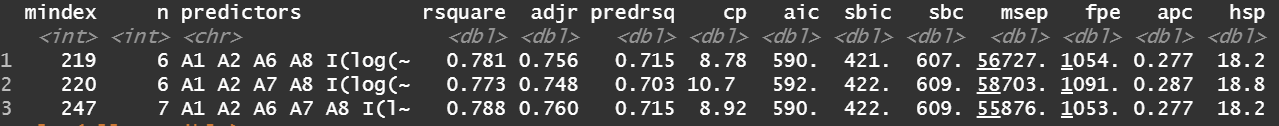
\includegraphics[width=\textwidth]{graphiques/Qst1_all_possible_models_top3}
		\caption{Résultats des trois meilleurs modèles selon la statistique du $R^2$ de prédiction.}
		\label{Qst1_all_possible_models_top3}
	\end{figure}
	Comme les modèles 219 et 247 sont très comparables, on choisira celui qui est le plus simple étant donné que le jeu de données d'entraînement comporte très peu d'observations (60). Ainsi, le modèle sélectionné est le suivant:
	\begin{equation}\label{modele_variables_selectionnees}
		\mathrm{B} \sim \mathrm{A1 + A2 + A6 + A8 + I(log(A13)) + I(sqrt(A9))}.
	\end{equation}
	À ce stade, il pourrait être intéressant de voir si des interactions entre les variables amélioreraient le pouvoir de prédiction. Pour identifier celles qui sont intéressantes, on applique le test F partiel sur toutes les interactions de 1er ordre possible. Se faisant, on trouve qu'aucune des interactions n'est significative au seuil de 1\%. Donc, le modèle \eqref{modele_variables_selectionnees} correspond à notre modèle final.\\
	
	Avec la fonction \texttt{ols\_regress} du \textit{package} \texttt{olsrr}, on peut calculer plusieurs statistiques d'intérêt pour décrire les performances du modèle final. D'une part, on a un $R^2$ de prédiction qui est de 71\%, ce qui est très bon considérant que la mortalité est un phénomène complexe auquel il est impossible de décrire à 100\% avec des variables explicatives. D'autre part, la statistique de Wald nous indique que chacune des variables explicatives incluses dans le modèle est significative à un seuil de 5\%.
	
	\subsection{Calcul de la prédiction}
	Maintenant que l'on a un modèle appréciable, on aimerait calculer un estimé ponctuel ainsi qu’un intervalle de confiance à 95\% pour le taux de mortalité à un endroit pour lequel les variables A1 à A15 valent respectivement
	\begin{center}
		40 30 80 9 3 10 77 4100 13 46 15 25 26 145 55.
	\end{center}
	Avec la fonction \texttt{predict} du \textit{package} \texttt{stats}, on obtient un estimé de $\hat{B} = 999.4799$ ainsi qu'un intervalle de prédiction correspondant à  $B \in [936.0751, 1062.885]$.
	
\section{Question 2}
	Pour la deuxième question de ce travail, on présente une base de données avec 13 variables explicatives, chacune mesurant une métrique médicales du corps humain. L'objectif est de construire un modèle de régression qui estime la probabilité de diagnostic positif pour la maladie coronarienne afin d'identifier les variables associées a une hausse du risque de développer la maladie.
	
	\subsection{Analyse préliminaire}
	D'abord, en jetant un œil sur les données, on se rend compte qu'un prétraitement est nécessaire. Effectivement, les variables \texttt{ca} et \texttt{thal} contiennent des points d'interrogation "\texttt{?}" puisque, pour certaines observations, ces métriques n'ont pas été calculées. Comme ces cas sont peu nombreux (6 observations), ils sont simplement écartés du jeu de données. D'autres modifications ont été apportées aux variables afin que le format des données soit cohérent avec leur nature. Pour plus de détail, voir le code informatique fournit en pièce jointe.
	
	
	\subsection{Traitement de la multicollinéarité}\label{sect_qst2_vif}
	Comme pour la première question, afin de construire un modèle de prédiction, la première étape est de réaliser une analyse de multicolinéarité conformément à la section \ref{sect_multicollinearite}.
	%
	Comme cette étape ne concerne que la matrice $\boldsymbol{X}$, il n'est pas nécessaire d'entraîner un GLM à ce stade pour réaliser cette analyse. Ainsi, il est possible d'utiliser la fonction \texttt{ols\_vif\_tol()} en entraînant un modèle linéaire sur une variable réponse bidon. Se faisant, on trouve qu'aucune variable explicative ne semble a priori dépendre linéairement des autres. Cependant, on se rappelle que, pour les variables catégorielles, cette méthode est peu fiable. Pour cette raison, on regarde également la métrique du VIF généralisé (GVIF). Comme
	$(\mathrm{GVIF}_j)^{1/(2 p_j)} < 3.16,$ pour $j=1,\dots,13$, alors on déduit qu'il n'y a pas de problème de multicolinéarité et on peut procéder à la sélection des variables explicatives.


	\subsection{Sélection des variables explicatives}\label{sect_qst2_selection_variables}	
	Pour cette question, comme la variable endogène est catégorielle, le type de modèle de régression sélectionné pour réaliser la tâche est le modèle linéaire généralisé de la famille binomiale. De plus, comme l'objectif est d'interpréter les paramètres du modèle, la fonction de lien retenue correspond à la fonction canonique, c.-à-d. la fonction logit.\\
	
	Dans un premier temps, avant de retirer des variables explicatives du modèle complet, il est pertinent de voir si certaines transformations appliquées sur les variables explicatives numériques pourraient améliorer l'explicabilité de la variable endogène. Pour se faire, on peut entraîner un modèle additif généralisé (GAM) à l'aide de la fonction \texttt{gam} qui provient du \textit{package} du même nom. Par la suite, il suffit de passer le modèle entraîné dans la fonction \texttt{plot} afin de visualiser graphiquement les transformations réalisées par la fonction \texttt{gam}. Si la courbe affichée est linéaire, cela signifie qu'aucune transformation n'est nécessaire. Autrement, la forme de la courbe donne une idée de la transformation à effectuer. Dans le cas présent, aucune transformation n'est nécessaire.\\

	Dans un deuxième temps, afin de sélectionner les variables explicatives, la fonction \texttt{glmbb} du \textit{package} du même nom permet de tester tous les sous-modèles possibles en utilisant l'AIC comme critère de performance. Après avoir exécuté cette fonction, on sélectionne les cinq modèles minimisant ce critère. Étant donné que l'objectif est d'expliquer un phénomène et non de réaliser une prédiction, les cinq modèles restant sont comparés à l'aide du la statistique du $R^2$ ajusté. Ainsi, on trouve que le meilleur modèle correspond à \eqref{modele_selectionnes_qst2}.
	\begin{equation}\label{modele_selectionnes_qst2}
		\mathrm{Y} \sim \mathrm{thal + ca + cp + oldpeak + slope + sex + trestbps + 
		exang + thalach}.
	\end{equation}
	
	Les méthodes algorithmiques d'inclusion (\textit{forward}), d'exclusion (\textit{backward}) et pas-à-pas (\textit{stepwise}) ont également été testées avec la fonction \texttt{stepAIC} du \textit{package} \texttt{MASS}; ce faisant, on obtient le même résultat dans tous les cas.\\
	
	On désire maintenant voir si des interactions amélioreraient l'explicabilité de la variable endogène. On procède donc avec la méthode pas-à-pas avec le test du ratio des vraisemblance pour un seuil d'inclusion et d'exclusion de 5\%. Ce faisant, on trouve le modèle \eqref{modele_final_q2}.
	\begin{align}\label{modele_final_q2}
		\mathrm{Y} &\sim \mathrm{sex + cp + trestbps + oldpeak + slope + ca + thal + ca:thal}.
	\end{align}		
	
	
	\subsection{Facteurs explicatifs}
	Afin de répondre a la question on analyse la sortie \texttt{R} de la fonction \texttt{summary} pour le modèle \eqref{modele_final_q2} tel que présenté dans l'illustration \ref{model_final_q2_sommaire}.
	\begin{figure}[H]
		\centering
		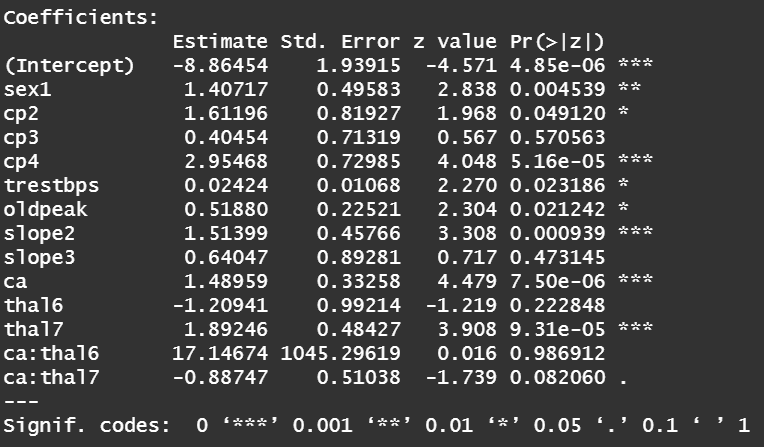
\includegraphics[width=0.6\textwidth]{graphiques/model_final_q2_sommaire}
		\caption{Sortie \texttt{R} de la fonction \texttt{summary} pour le modèle \eqref{modele_final_q2}.}
		\label{model_final_q2_sommaire}
	\end{figure}

	La première chose que l'on remarque dans l'illustration \ref{model_final_q2_sommaire}, c'est que l'écart-type de l'estimateur associé à l'interaction \texttt{ca:thal6} est démesurément grand. Pourtant, une analyse de la multicollinéarité ne soulève aucun problème. On en déduit que cette variable n'est pas utile et pourrait probablement être regroupée avec \texttt{thal3}. Dans ce cas, l'interprétation de la variable \texttt{thal} ainsi modifiée serait que le défaut soit réparable ou non.
	Si on procède à cette modification, le sommaire du modèle devient tel que présenté dans l'illustration \ref{model_final_q2_sommaire_2}.
	\begin{figure}[H]
		\centering
		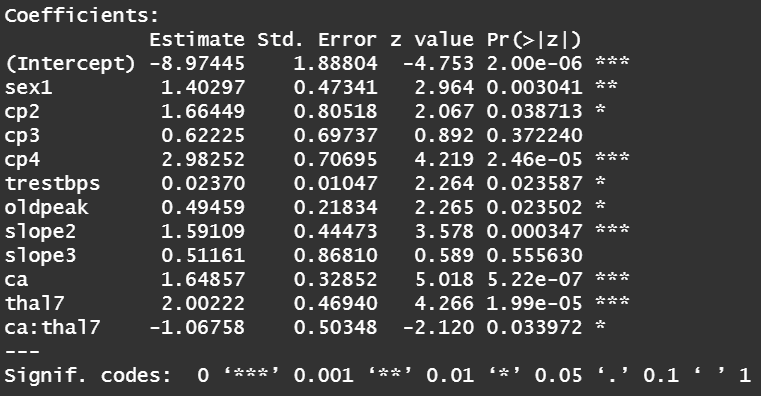
\includegraphics[width=0.6\textwidth]{graphiques/model_final_q2_sommaire_2}
		\caption{Sortie \texttt{R} de la fonction \texttt{summary} pour le modèle \eqref{modele_final_q2} lorsque les classes 3 et 6 sont regroupées pour la variable catégorielle \texttt{thal}.}
		\label{model_final_q2_sommaire_2}
	\end{figure}
	Désormais, toutes les classes de la variable \textit{thal} et de son interaction sont significative au seuil de 5\% selon le test de Wald et le problème de l'écart-type démesuré est réglé. On peut donc procéder à l'analyse de l'association des variables explicatives avec la variable endogène.\\

	Soit $\pi$, la probabilité qu'un diagnostic de maladie coronarienne soit positif. On a
	$$\pi = \mathrm{logistique}(\eta) = \mathrm{logit}^{-1}(\eta) = \frac{e^{\eta}}{1+e^\eta},$$
	où $\eta = \boldsymbol{x'\beta}$ et $\boldsymbol{x'\beta}$ est représentée par \eqref{modele_final_q2}.
	Par dérivation en chaîne, on a 
	\begin{align}\label{eq_derivee_pi}
		\frac{\partial\pi}{\partial \boldsymbol{\beta}} 
		= \frac{\partial\pi}{\partial \eta}\frac{\partial\eta}{\partial \boldsymbol{\beta}}
		= \frac{e^\eta (1+e^\eta) - e^{2\eta}}{(1+e^\eta)^2} \boldsymbol{x}
		= \frac{e^\eta}{(1+e^\eta)^2}\boldsymbol{x} 
		= \pi(1-\pi)\boldsymbol{x}.
	\end{align}
	Comme $\pi\in[0,1]$, alors $\pi(1-\pi)\in[0,1]$. Ainsi, si $\boldsymbol{x}$ est un vecteur de valeurs positives, on déduit avec \eqref{eq_derivee_pi} que la fonction logistique est croissante par rapport aux coefficients.
	%
	Cela signifie que si on augmente une variable explicative d'une unité, la prédiction de la probabilité de diagnostic positif augmentera si le coefficient visé est positif et elle diminuera dans le cas contraire.
	%
	Conséquemment, les variables exogènes ayant un estimateur positifs seront associées à une hausse du risque d'un diagnostic positif de maladie coronarienne. Ces dernières sont: 
	\begin{itemize}
		\item \texttt{sex}: le sexe,
		\item \texttt{cp}: la nature des douleurs à la poitrine,
		\item \texttt{trestbps}: la tension artérielle au repos,
		\item \texttt{oldpeak}: la baisse du segment ST induite par l’exercice par rapport au repos,
		\item \texttt{slope}: la pente du segment ST lors de l’exercice maximal.
	\end{itemize}

	En ce qui attrait aux variables explicatives \texttt{ca} et \texttt{thal}, l'association positive est moins claire étant donnée l'interaction qui existe entre elles. En effet, les coefficients associés à ces variables sont donnés respectivement par \eqref{eq_coefficient_ca} et \eqref{eq_coefficient_thal} .
	\begin{align}\label{eq_coefficient_ca}
		\left( 1.64857 -1.06758  \times \texttt{thal7}\right)
	\end{align}
	\begin{align}\label{eq_coefficient_thal}
		\left(2.00222 -1.06758  \times \texttt{ca}\right)
	\end{align}
	On voit donc avec \eqref{eq_coefficient_ca} que le coefficient de \texttt{ca} est toujours positif, peu importe la valeur de  \texttt{thal7} puisque $1.64857 -1.06758 > 0$. Cependant, pour \texttt{thal7}, la polarité du coefficient dépendra de la valeur de \texttt{ca} puisque \texttt{ca} $\in \{0, 1, 2, 3\}$.
	
	
\section{Question 3}
	Pour cette question, on utilise le jeu de données \texttt{ausprivauto0405} disponible sur le \textit{package} \texttt{R CASdatasets}. Celui-ci contient des données sur les polices d'assurance automobile d'une durée d'un an contractées en Australie entre 2004 et 2005. On y trouve trois caractéristiques du véhicule assuré et deux autres relatives au détenteur de police. On y voit aussi l'exposition (proportion de l'année où la police est active) et le nombre d'accidents survenus lors de la couverture de la police.
	%
	L’objectif est de construire un modèle de régression qui permettrait d'identifier les variables ayant une association significatives avec le nombre de réclamations.
	%
	Puisque la variable endogène correspond à un dénombrement, un GLM Poisson est choisi pour réaliser la tâche. Afin de simplifier le modèle et l'interprétation, la fonction de lien log est retenue. Par ailleurs, puisque le dénombrement des accidents est proportionnel à l'exposition, on utilisera cette dernière variable comme terme d'\textit{offset}.
	
	
	\subsection{Traitement de la multicollinéarité}
	Comme dans la section \ref{sect_qst2_vif}, on est en présence de plusieurs variables catégorielles. Conséquemment, la métrique appropriée pour vérifier la multicolinéarité est le VIF généralisé qui est calculé avec la fonction \texttt{vif} du \textit{package} \texttt{car}.
	Comme $(\mathrm{GVIF}_j)^{1/(2p_j)} < 3, j=1,2,\dots,5,$ alors on déduit qu'il n'y a pas de problème de multicolinéarité.

	
	\subsection{Traitement de la surdispersion}
	On sait que la loi de Poisson a une espérance égale à sa variance. En termes des lois de la famille exponentielle, cela implique que le paramètre de dispersion $\phi$ doit être très près de 1.
	Or, l'estimateur de la méthode des moments de ce paramètre, qui est calculé à l'aide de \eqref{estimateur_parametre_dispersion}, donne une valeur de $0.373606$. On déduit donc que le modèle est sous-dispersé.
	\begin{equation}\label{estimateur_parametre_dispersion}
		\hat{\phi}_D = D(\boldsymbol{y};\hat{\boldsymbol{\mu}})/(n-p),
	\end{equation}
	où $D(\boldsymbol{y};\hat{\boldsymbol{\mu}})$ correspond à la statistique de déviance du modèle, $n$ représente le nombre d'observations, soit $n=67\,856$, et $p$ correspond au nombre de paramètres du modèle, soit $p=23$.
	%
	La façon la plus commune de traiter les données de dénombrement avec variabilité extra-poissonienne est de supposer un modèle de type binomiale négative.
	%
	Étant donnée que le modèle de Poisson est une simplification du modèle binomial négative (paramètre $\alpha=0$ dans le cas poissonien), on peut procéder au test du ratio des vraisemblances pour déterminer si le modèle binomial négative améliore significativement la vraisemblance par rapport au GLM Poisson. Cependant comme le test d'hypothèse est hors norme (le test d'hypothèse est unilatéral), il faut adapter le calcul du seuil observé avec \eqref{Pvalue_LRT_surdispersion}.
	\begin{equation}\label{Pvalue_LRT_surdispersion}
		p_{\mathrm{value}} = 0.5\times \P[\chi^2_1 > 2(l_1 - l_0)],
	\end{equation}
	où $l_1$ et $l_0$ correspondent respectivement à la log-vraisemblance pour le modèle complet (binomial négative) et pour le modèle simplifié (Poisson).
	Ainsi, en calculant \eqref{Pvalue_LRT_surdispersion} sur le jeu de données, on trouve un seuil observé de 
	$1.904829\times 10^{-10}$. On rejette donc l'hypothèse nulle que le modèle de Poisson est suffisant pour conclure que le modèle binomial négative est mieux adapté aux données.
	
	
	\subsection{Sélection des variables explicatives}
	Dans un premier temps, afin de vérifier si une transformation de la variable \texttt{VehValue} améliorerait le modèle, on peut utiliser la fonction \texttt{gam} comme dans la section \ref{sect_qst2_selection_variables}. Se faisant, on réalise que non, aucune transformation n'est requise.\\
	
	Par la suite, pour faire la sélection des variables explicatives, il aurait été idéal de tester tous les sous-modèles possibles pour sélectionner celui qui maximise l'explicabilité de la variable endogène. Cependant, avec \texttt{R}, la fonction \texttt{glmbb} ne peut être appliqué avec la loi binomiale négative. 
	%
	La fonction \texttt{glmulti} provenant du \textit{package} du même nom nécessite l'installation de \texttt{JavaScript}. Pour les fins de ce travail, afin d'éviter des difficultés de correction, nous avons décidé de ne pas tester la fonction.
	%
	Pour ces raisons, les méthodes algorithmiques ont été privilégiées. Ainsi, la fonction \texttt{stepAIC} du \textit{package} \texttt{MASS} permet de trouver le modèle \eqref{modele_selectionne_qst3}, peu importe qu'on soit sous l'approche d'inclusion, d'exclusion ou pas-à-pas.
	\begin{equation}\label{modele_selectionne_qst3}
		\mathrm{ClaimNb} \sim \mathrm{DrivAge + VehAge + VehBody + offset(log(Exposure))}.
	\end{equation}
	
	Il ne reste plus qu'à regarder si l'inclusion d'une interaction améliorerait les performances du modèle.
	Avec un test du ratio de vraisemblance, on trouve qu'aucune interaction n'est significative au seuil de 5\%.
	
	\subsection{Description du modèle final}
	Dans un premier temps, on s'intéresse à savoir quelles variables contribuent à augmenter l'espérance du nombre de sinistres automobiles qui surviennent dans une année. Pour se faire, on peut calculer la dérivée première de cette espérance par rapport aux coefficients de régression.
	Soit $\mu$, l'espérance du nombre d'accidents automobiles survenus dans une année. Avec le lien log, on a
	\begin{equation}\label{lien_log}
		\mu = e^{\eta},
	\end{equation} 
	où $\eta = \boldsymbol{x'\beta}$ et $\boldsymbol{x'\beta}$ est représenté par \eqref{modele_selectionne_qst3}. Par dérivation en chaîne, on a
	\begin{align}\label{derivee_mu}
		\frac{\partial \mu}{\partial \boldsymbol{\beta}} = \frac{\partial \mu}{\partial \eta}\frac{\partial \eta}{\partial \boldsymbol{\beta}} = e^\eta \boldsymbol{x} = \mu\boldsymbol{x}.
	\end{align}
	Comme $\mu\geq0$, alors, si $\boldsymbol{x}$ est un vecteur de valeurs positives, on déduit avec \eqref{derivee_mu} que l'espérance du nombre de sinistres survenus dans une année est une fonction croissante par rapport aux coefficients de la régression.\\
	
	L'un des grands avantages de la fonction de lien log pour la régression de Poisson et binomiale négative, c'est sa facilité d'interprétation. En effet, si une variable $x_j$ augmente d'une unité, alors l'espérance du nombre d'accident dans une année sera multipliée par $e^{\beta_j}$. Ces valeurs multiplicatives sont calculées pour chacune des variables explicatives dans les tableaux \ref{facteurs_multiplicatifs_DriveAge} à \ref{facteurs_multiplicatifs_VehAge}.\\
	
	Dans un premier temps, interprétons ce que le coefficient $\hat{\beta}_0$ veut dire dans le modèle.
	Dans cette situation, on considère un assuré relativement âgé (\texttt{old people}), qui conduit un vieux  bus. Dans ce cas, l'espérance du nombre d'accident pour ce genre d'assuré, pour une année, est de $e^{-1.17389} \approx 0.309$. Par la suite, les facteurs présentés dans les tableaux \ref{facteurs_multiplicatifs_DriveAge} à \ref{facteurs_multiplicatifs_VehAge} viennent augmenter ou diminuer cette espérance selon les caractéristiques de l'assuré et de son véhicule.
	
	\begin{table}[H]
		\centering
		\begin{tabular}{lr}
			\hline
			Variables & Facteurs \\ 
			\hline
			DrivAgeoldest people & 1.01 \\ 
			DrivAgeolder work. people & 1.25 \\ 
			DrivAgeworking people & 1.28 \\ 
			DrivAgeyoung people & 1.36 \\ 
			DrivAgeyoungest people & 1.62 \\ 
			\hline
		\end{tabular}
		\caption{Facteurs multiplicatifs pour la variable \texttt{DriveAge}.}
		\label{facteurs_multiplicatifs_DriveAge}
	\end{table}
	Lorsque l'on regarde la variable \texttt{DriveAge}, on voit que la catégorie d'âge des assurés qui est la moins risquée correspond aux gens âgés (\texttt{old people}) et qui est associée au coefficient $\beta_0$. La catégorie d'âge la plus risquée, quant à elle, correspond aux plus jeunes conducteurs (\texttt{youngest people}) puisque le facteur multiplicatif correspondant est le plus élevé. On remarque que le risque diminue tandis que l'âge augmente jusqu'à ce que l'on arrive à un âge très respectable (\texttt{oldest people}). Dans ce cas, le risque réaugmente étant donnée que les réflexes du conducteur diminuent, de même que sa vision.

	\begin{table}[H]
		\centering
		\begin{tabular}{lr}
			\hline
			Variables & Facteurs \\ 
			\hline
			VehBodyConvertible & 0.22 \\ 
			VehBodyUtility & 0.33 \\ 
			VehBodyHatchback & 0.37 \\ 
			VehBodyMinibus & 0.38 \\ 
			VehBodyTruck & 0.38 \\ 
			VehBodySedan & 0.40 \\ 
			VehBodyStation wagon & 0.41 \\ 
			VehBodyPanel van & 0.42 \\ 
			VehBodyHardtop & 0.44 \\ 
			VehBodyRoadster & 0.59 \\ 
			VehBodyCoupe & 0.61 \\ 
			VehBodyMotorized caravan & 0.71 \\ 
			\hline
		\end{tabular}
		\caption{Facteurs multiplicatifs pour la variable \texttt{VehBody}.}
		\label{facteurs_multiplicatifs_VehBody}
	\end{table}
	Du point de vue du type de véhicule, on voit que la classe qui maximise l'espérance du nombre d'accident est le bus (associé à l'estimateur $\beta_0$) puisque tous les facteurs multiplicatifs sont inférieurs à 1. Le type de véhicule qui minimise cette espérance est le convertible. Si on analyse ces résultats plus en profondeur, on remarque que les véhicules les plus risqués, mis à part le bus, sont des véhicules sports (\texttt{roadster}, \texttt{coupe}) et ceux minimisant le risque sont des véhicules généralement conduits par des retraités (\texttt{convertibles}). Ainsi, bien que nous n'ayons pas observé d'interaction significative avec le test du rapport des vraisemblances, on remarque que certaines catégories de véhicule pourraient être associées à des groupes d'âge.

	\begin{table}[H]
		\centering
		\begin{tabular}{lr}
			\hline
			Variables & Facteurs \\ 
			\hline
			VehAgeoldest cars & 0.93 \\ 
			VehAgeyoungest cars & 1.09 \\ 
			VehAgeyoung cars & 1.14 \\ 
			\hline
		\end{tabular}
		\caption{Facteurs multiplicatifs pour la variable \texttt{VehAge}.}
		\label{facteurs_multiplicatifs_VehAge}
	\end{table}
	
	Finalement, en ce qui attrait à l'âge du véhicule, on a que la classe associée au coefficient $\beta_0$ est \texttt{old cars}. La classe la plus risquée est attribuée à \texttt{young cars} et celle qui est la moins sujette à un nombre élevé d'accident est \texttt{oldest cars}.\\
	
	On remarquera que le modèle final n'inclut pas la valeur relative du véhicule (\texttt{VehValue}). Si on applique un test du ratio des vraisemblances, on remarque que le seuil observé est de 0.1782. Comme ce seuil est très élevé, on déduit que cette variable n'est pas utile pour prédire le nombre d'accidents automobiles. En revanche, elle aurait pu être significative si on avait étudié le montant des sinistres. Dans ce cas, la valeur du véhicule aurait pu être utilisée comme variable d'exposition.
	
	
	\bibliographystyle{apalike}
	\bibliography{BibGLM}	
	
%	\clearpage
	\appendix
	\section{Illustrations}
	\begin{figure}[H]
		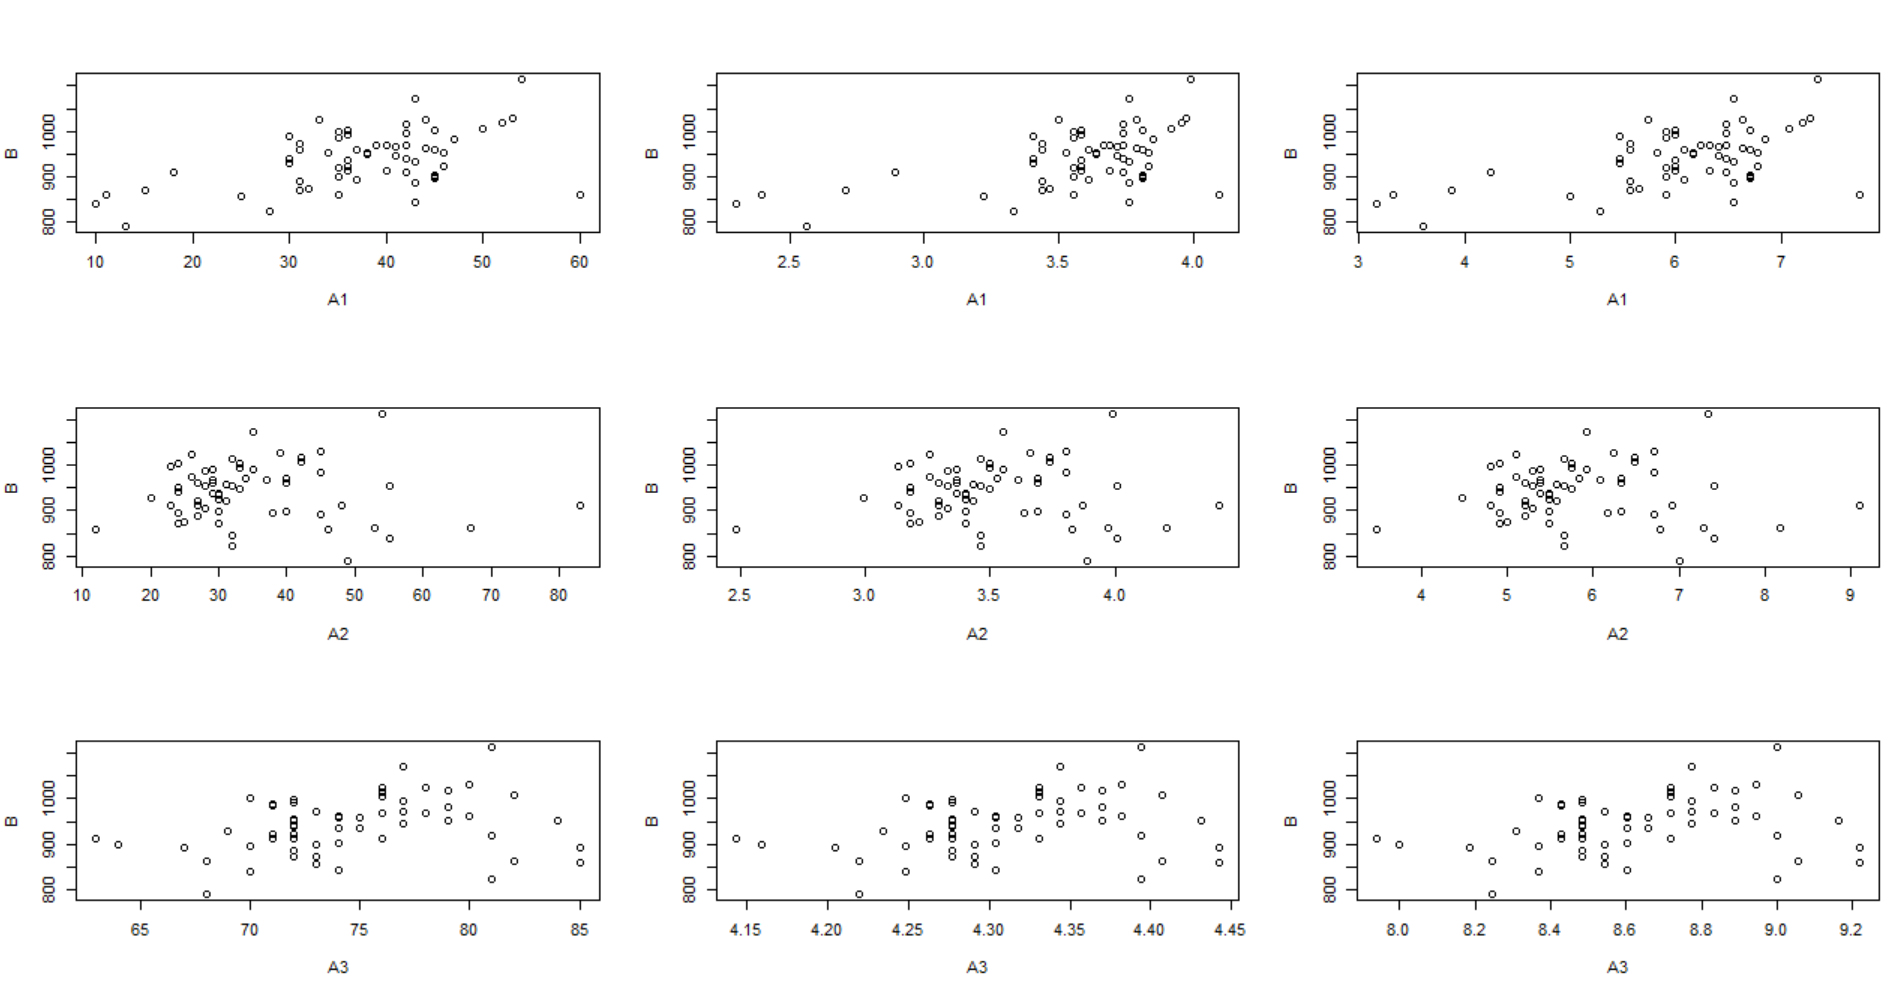
\includegraphics[width=\textwidth]{graphiques/Qst1_transformations_1}
		\caption{À gauche, on compare la variable endogène B avec les variables exogènes A1 à A3. Au centre, on compare la même relation, mais avec une transformation logarithmique effectuée sur les variables exogènes. À droite, c'est la transformation racine carrée qui est appliquée.}
		\label{Qst1_transformations_1}
	\end{figure}
	\begin{figure}[H]
		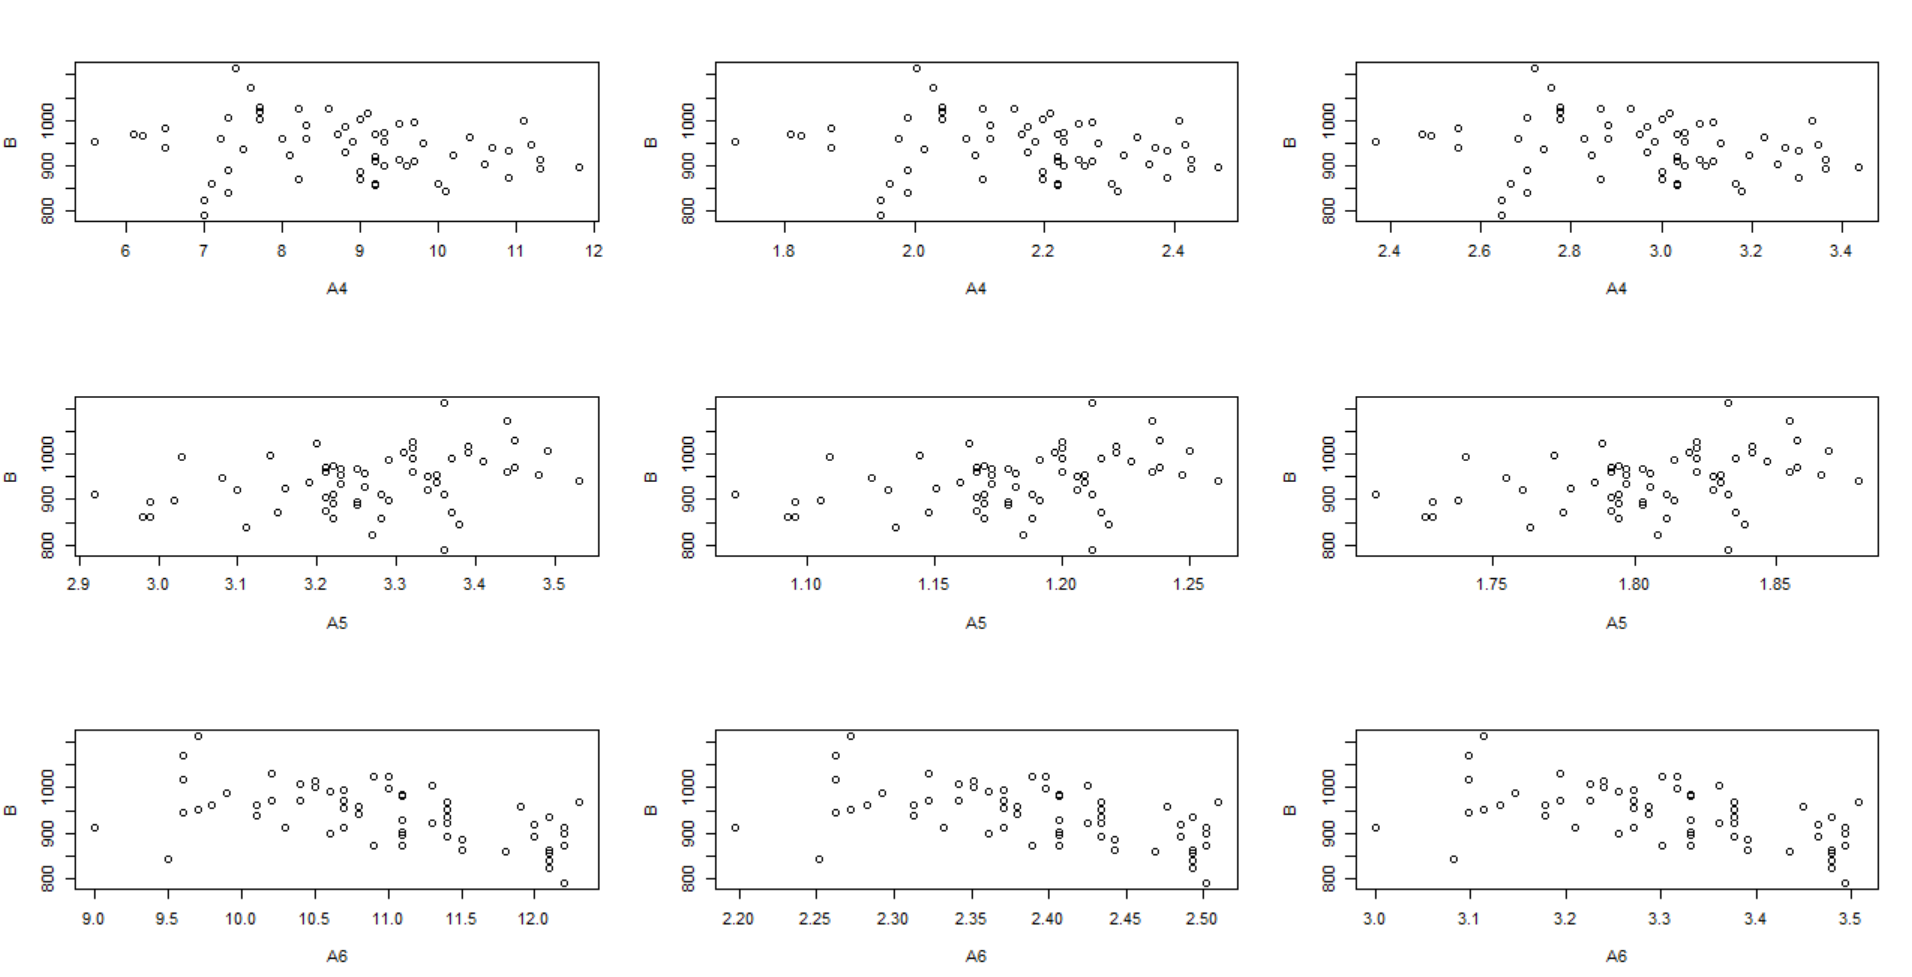
\includegraphics[width=\textwidth]{graphiques/Qst1_transformations_2}
		\caption{À gauche, on compare la variable endogène B avec les variables exogènes A4 à A6. Au centre, on compare la même relation, mais avec une transformation logarithmique effectuée sur les variables exogènes. À droite, c'est la transformation racine carrée qui est appliquée.}
		\label{Qst1_transformations_2}
	\end{figure}
	\begin{figure}[H]
		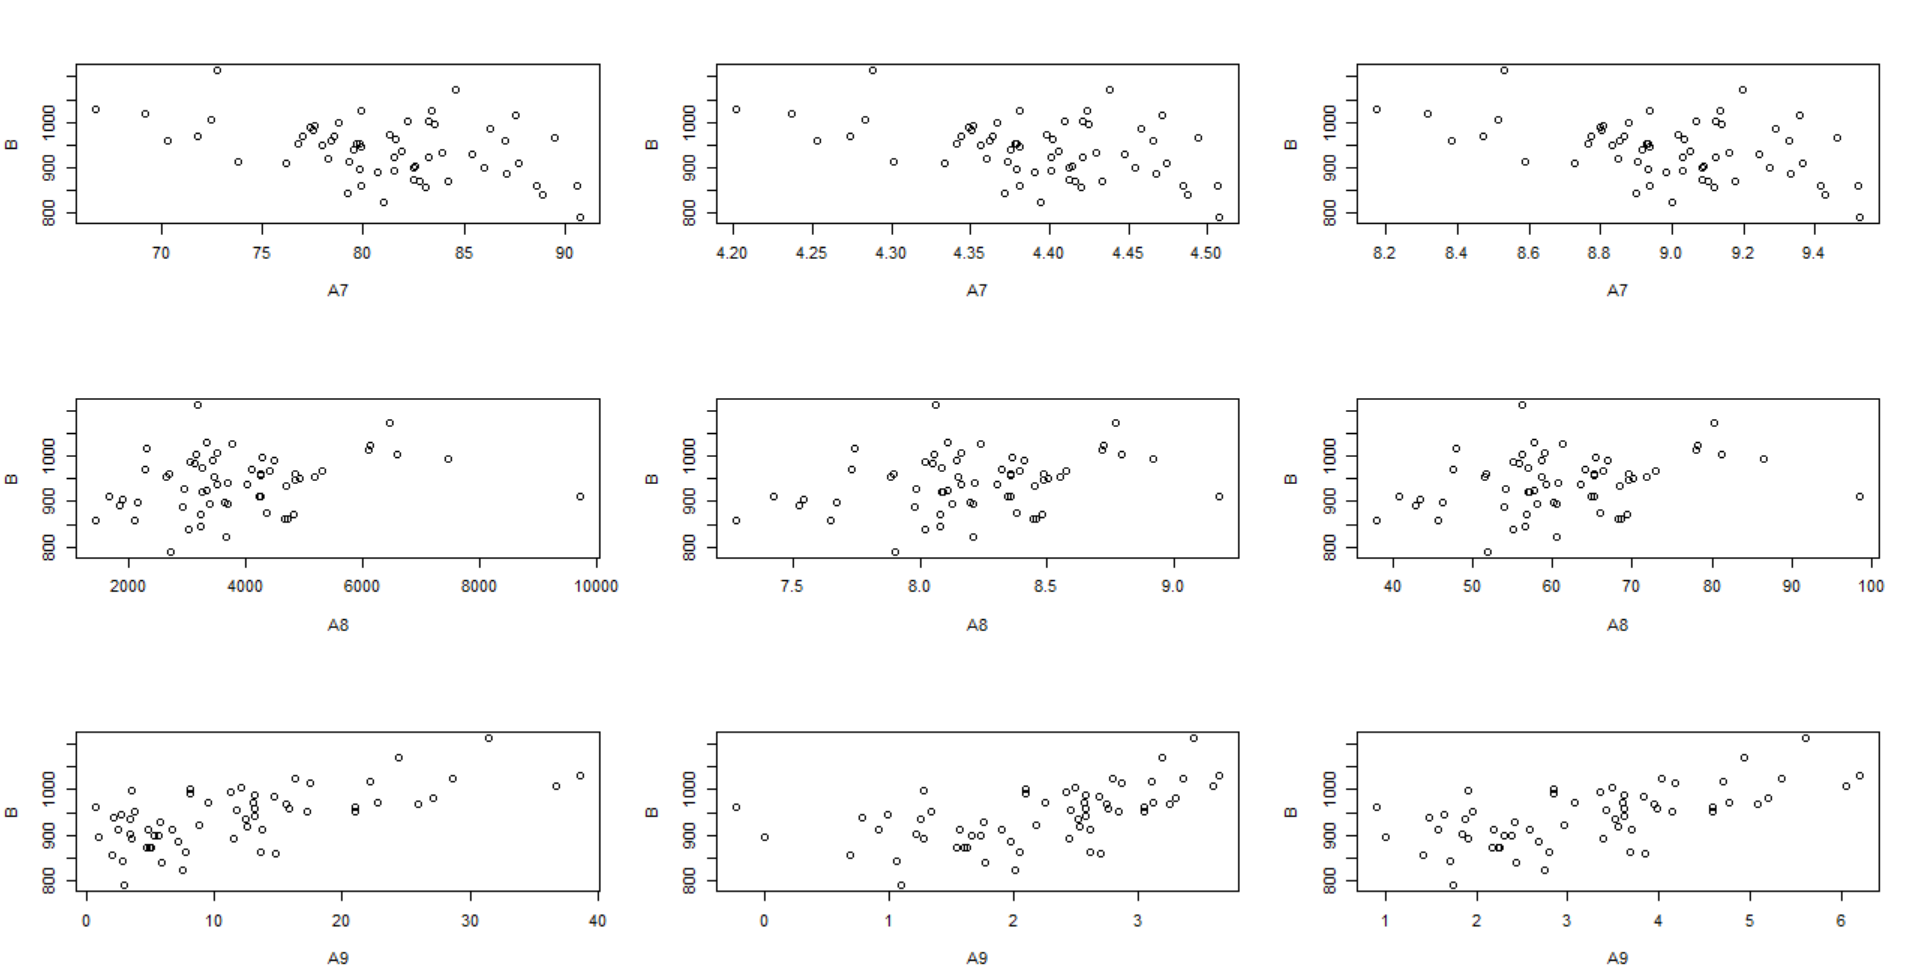
\includegraphics[width=\textwidth]{graphiques/Qst1_transformations_3}
		\caption{À gauche, on compare la variable endogène B avec les variables exogènes A7 à A9. Au centre, on compare la même relation, mais avec une transformation logarithmique effectuée sur les variables exogènes. À droite, c'est la transformation racine carrée qui est appliquée.}
		\label{Qst1_transformations_3}
	\end{figure}
	\begin{figure}[H]
		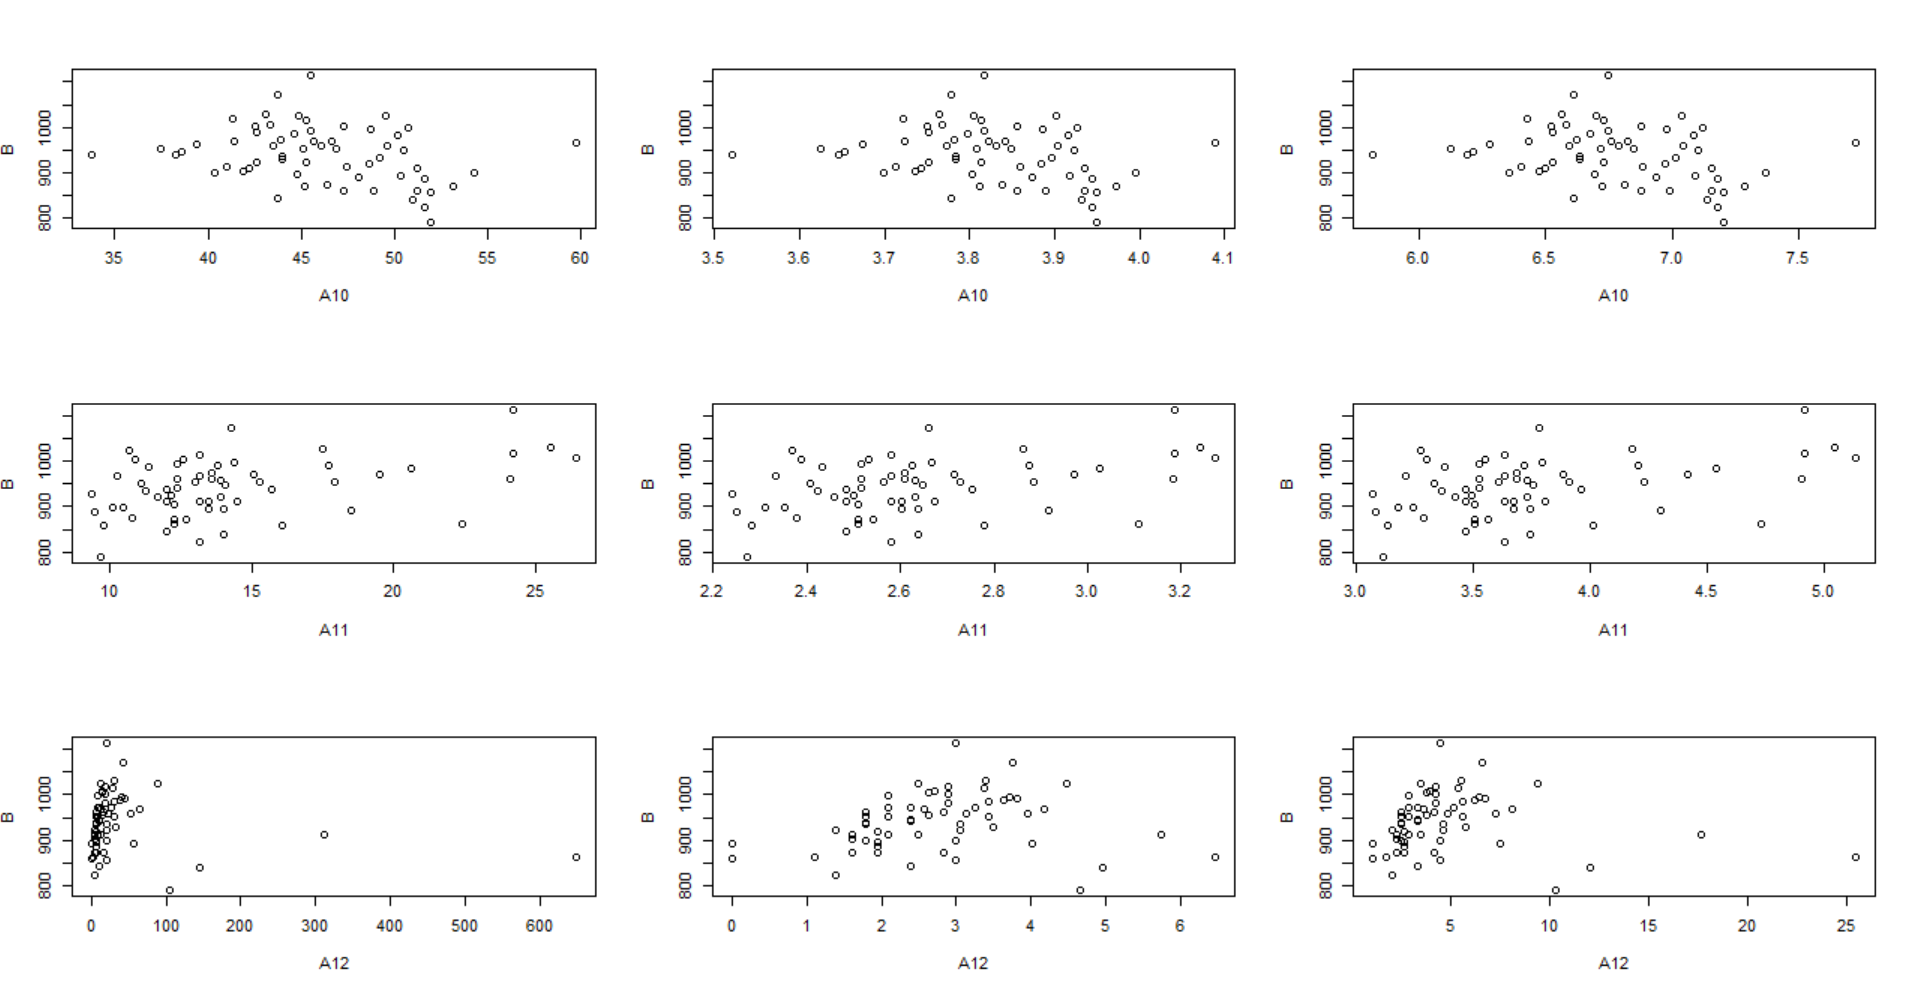
\includegraphics[width=\textwidth]{graphiques/Qst1_transformations_4}
		\caption{À gauche, on compare la variable endogène B avec les variables exogènes A10 à A12. Au centre, on compare la même relation, mais avec une transformation logarithmique effectuée sur les variables exogènes. À droite, c'est la transformation racine carrée qui est appliquée.}
		\label{Qst1_transformations_4}
	\end{figure}
	\begin{figure}[H]
		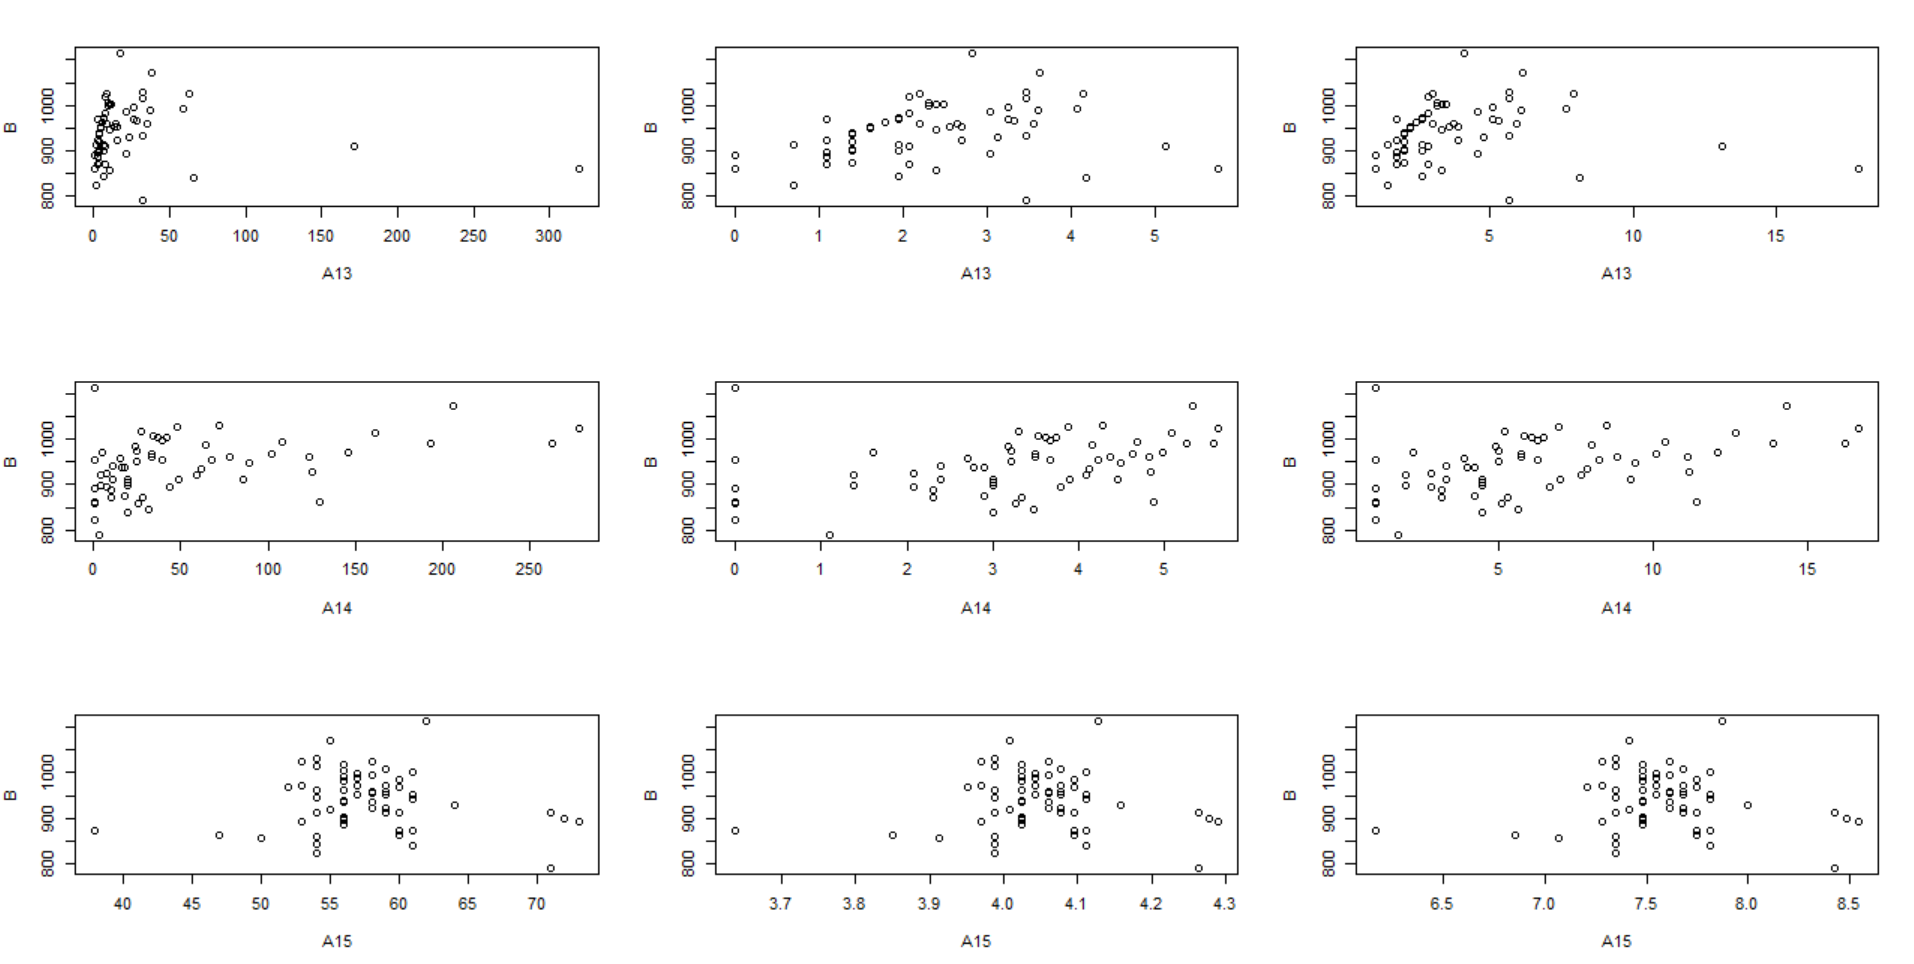
\includegraphics[width=\textwidth]{graphiques/Qst1_transformations_5}
		\caption{À gauche, on compare la variable endogène B avec les variables exogènes A13 à A15. Au centre, on compare la même relation, mais avec une transformation logarithmique effectuée sur les variables exogènes. À droite, c'est la transformation racine carrée qui est appliquée.}
		\label{Qst1_transformations_5}
	\end{figure}

%	\begin{figure}[H]
%		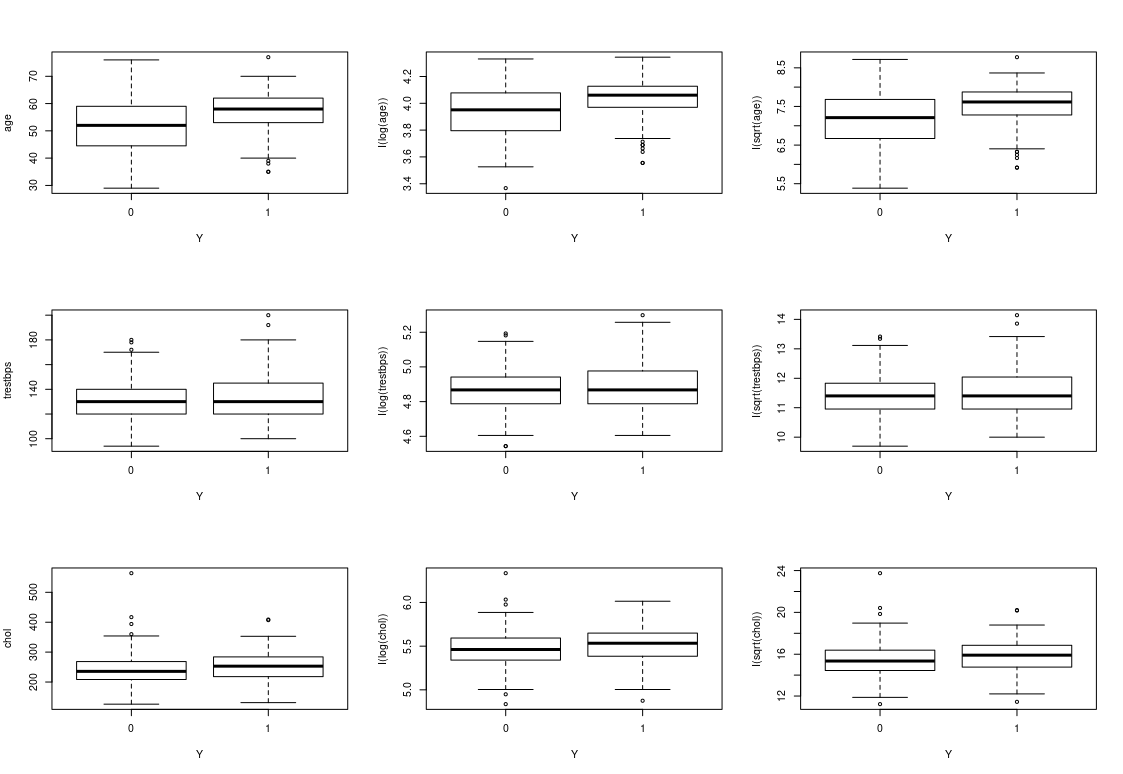
\includegraphics[width=\textwidth]{graphiques/Q2_transformation_1}
%		\caption{Boites a moustache entre la variables explicative et la variable dépendante Y.
%		À gauche, on compare la variable endogène Y avec les variables exogènes. Au centre, on compare la même relation, mais avec une transformation logarithmique effectuée sur les variables exogènes. À droite, c'est la transformation racine carrée qui est appliquée.}
%		\label{Q2_transformations_1}
%	\end{figure}
%
%	\begin{figure}[H]
%		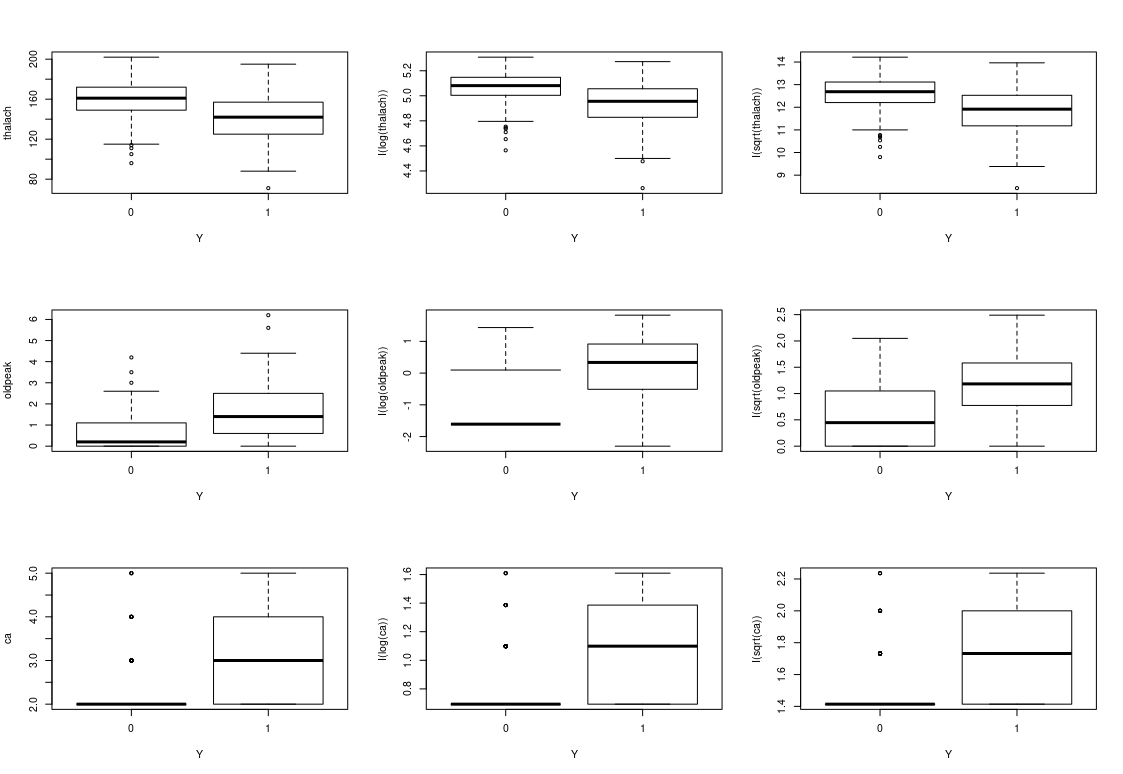
\includegraphics[width=\textwidth]{graphiques/Q2_transformation_2}
%		\caption{Boites a moustache entre la variables explicative et la variable dépendante Y.
%			À gauche, on compare la variable endogène Y avec les variables exogènes. Au centre, on compare la même relation, mais avec une transformation logarithmique effectuée sur les variables exogènes. À droite, c'est la transformation racine carrée qui est appliquée.}
%		\label{Q2_transformations_2}
%	\end{figure}
	

	
	
\end{document}